\section{Arithmetic Programs}
Suppose we have some algebra \(\mathbb{A}\): we can represent and deal with finite sequences of 
operations, called \emph{expressions}, between elements of \(\mathbb{A}\) and/or variables over 
\(\mathbb{A}\).

For example, given the expression \(x^2 + x + 1\) over \(\mathbb{R}\left[x\right]\), we might be 
interested to know what is the \emph{evaluation} of the expression given some value for \(x\).

\begin{definition}[Arithmetic formula]
  Given an algebraic structure \(\mathbb{A} = \Tuple{A, \odot_1, \dots, \odot_n}\), an explicit 
  arithmetic formula over \(\mathbb{A}\) is any expression \(\varphi \) of the kind:
  \begin{align*}
    & \varphi \equiv a && \textnormal{with \(a\) constant over \(A\)} \\ 
    & \varphi \equiv x && \textnormal{with \(x\) variable over \(A\)} \\
    & \varphi \equiv \call{\odot_i}{\varphi_1, \dots, \varphi_{\abs{\odot_i}}} && 
    \textnormal{with \(\varphi_1, \dots, \varphi_{\abs{\odot_i}}\) formulae over \(A\)}
  \end{align*}
  Additionally, an implicit (or succint) arithmetic formula also allows expressions involving 
  exponentiation:
  \begin{align*}
    & \varphi \equiv \call{\odot_i^k}{\varphi_1} && 
    \textnormal{\(\forall k \in \mathbb{N}\), with \(\varphi_1\) formula over \(A\)}
  \end{align*}
  where \(\odot_i^k\) represents the \(k\)th power of \(\odot_i \). 
\end{definition}

\begin{remark}
  It is always possible to translate an implicit formula into an equivalent explicit one.
  We denote the explicit version of an implciit formula \(\varphi \) with \(\explicit{\varphi}\).
  For some particular structures, such as fields, this translation can be specialized. 
\end{remark}

From now on, we will only deal with arithmetic formulae over some field (or ring) \(\mathbb{F}\), 
in which case implicit arithmetic expressions are equivalent to multi-variate polynomials.
\begin{example}\label{ex:arithmetic_formula}
  Consider the finite field \(\mathbb{Z}_{13}\).
  For ease of notation, we will use \(+\), juxtaposition and superscripting to denote, respectively,
  field addition, field multiplication, and exponentiation w.r.t.\ field multiplication. 
  A possible implicit arithemtic formula over \(\mathbb{Z}_{13}\) is the following expression:
  \[\varphi = x_{2}\Parens*{x_{1}^{3} + 4x_{2} + 5}\]
  Since in a finite field multiplication by a constant is simply repeated addition, i.e. 
  \(cx = \call{+^{c}}{x}\), the explicit version of \(\varphi \) then is:
  \[\explicit{\varphi} = x_{2}\Parens*{x_{1}x_{1}x_{1} + x_{2} + x_{2} + x_{2} + x_{2} + 5}\]
\end{example} 

\subsection{Arithmetic circuits}
It is possible to visually represent an arithmetic formula using a particualr kind of labeled 
\emph{directed acyclic graph} (DAG), called the \emph{arithmetic circuit}.
\begin{definition}[Arithmetic circuit]
  An arithmetic circuit over an algebra \(\mathbb{A} = \Tuple{A, \odot_1, \dots, \odot_n}\) and a 
  set of variables \(X\) over \(\mathbb{A}\) is a triple \(\mathcal{G} = \Tuple{V, E, L}\) where 
  \(V\) is the set of \emph{vertices}, \(E \subseteq V \times V\) is the set of \emph{edges}, and 
  \(L\colon V \to A \cup X \cup \Parens*{\Set{\odot_1, \dots, \odot_n} \times \mathbb{N}}\) is 
  the vertex \emph{labeling map}, such that, \(\forall v \in V\):
  \begin{align*}
    & \call{L}{v} \in A && \implies \nexists w \in V\colon \Tuple{w, v} \in E
    && \textnormal{(no in-edges for constant nodes)} \\
    & \call{L}{v} \in X && \implies \nexists w \in V\colon \Tuple{w, v} \in E
    && \textnormal{(no in-edges for variable nodes)} \\
    & \forall i \le n\colon \odot_i \in \call{L}{v} && \implies \abs{\Set{\Tuple{w, v}}_{w \in V} \cap E} = \abs{\odot_i}
    && \textnormal{(exactly \(\abs{\odot_i}\) in-edges for \(\odot_i\) nodes)}
  \end{align*}
\end{definition}

As an abuse of notation, we will sometimes identify a node \(v\) with its label \(\call{L}{v}\).
Given any explicit arithmetic formula \(\varphi \) over an algebra \(\mathbb{A}\) and a set of 
variables \(X\), we can build the corresponding arithmetic circuit \(\mathcal{G} = \Tuple{V, E, L}\) 
in the following way: for every distinct (i.e.\ ignoring repetitions) variable \(x\) appearing 
in \(\varphi \), we add a vertex \(v\) with label \(\call{L}{v} = x\); 
for every distinct constant \(c\) appearing in \(\varphi \) we add a vertex \(v\) with label 
\(\call{L}{v} = c\); 
finally, for every occurence \(i\) of some operation \(\odot \) in \(\varphi \), we add a vertex
\(v\) with label \(\call{L}{v} = \odot_{i}\).
Furthermore, we can partition \(V\) as follows:
\begin{itemize}
  \item \emph{Constant vertices}: 
    \(\mathcal{G}_{const} = \Set{v \mid \call{L}{v} \in \mathbb{A}}\) .
  \item \emph{Variable vertices}: 
    \(\mathcal{G}_{var} = \Set{v \mid \call{L}{v} \in X}\).
  \item \emph{Operation vertices}: 
    \(\mathcal{G}_{\odot_i} = \Set{v \mid \odot_i \in \call{L}{v}}\).
  \item \emph{Input vertices}: 
    \(\mathcal{G}_{in} = \mathcal{G}_{const} \cup \mathcal{G}_{var}\).
  \item \emph{Output vertices}: 
    \(\mathcal{G}_{out} = \Set{v \mid \nexists w \in V\colon \Tuple{v, w} \in E}\).
  \item \emph{I/O vertices}: \(\mathcal{G}_{IO} = \mathcal{G}_{in} \cup \mathcal{G}_{out}\).
\end{itemize}

To build the set of edges \(E\), for every operation occuring in \(\varphi \), we connect the 
vertices representing the operands to the vertex representing said operation, e.g.\ if we have 
the formula \(\Parens*{x \odot y} \odot z\) we add the edges \(\Tuple{x, \odot_1}\), 
\(\Tuple{y, \odot_1}\) and \(\Tuple{z, \odot_2}\).
We also consider operation nodes as holding the intermediate values of the computation: in the 
previous example, we will also have the edge \(\Tuple{\odot_1, \odot_2}\), where \(\odot_1 \) 
represents the intermediate value \(x \odot y\).
The fact that we store all the intermediate values of a computation is something that can be 
greatly exploited to optimize the design of a circuit.

\begin{example}
  \Cref{fig:arithmetic_circuit} shows the arithmetic circuit derived from the formula shown in 
  \Cref{ex:arithmetic_formula}.
  We can see the two variable vertices \(x_1\) and \(x_2\) which are also input vertices, the 
  constant vertex \(5\), which is an input vertex too, the
  addition vertices \(\oplus_1, \dots, \oplus_5\) and the multiplication vertices 
  \(\otimes_1, \otimes_2, \otimes_3\), of which the latter is also an output vertex.
\end{example}

\begin{figure}
	\centering
	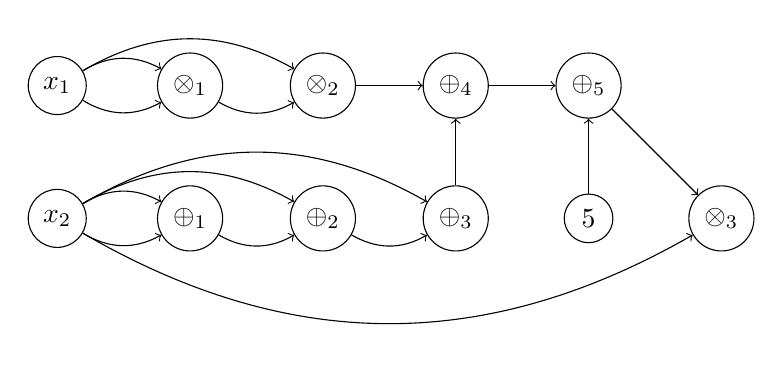
\begin{tikzpicture}[node distance={48pt}, node/.style = {draw, circle}]
		\node[node] (x1) {\(x_1\)};
		\node[node] (x2) [below of=x1] {\(x_2\)};
		\node[node] (m1) [right of=x1] {\(\otimes_1\)};
		\node[node] (m2) [right of=m1] {\(\otimes_2\)};
		\node[node] (a1) [right of=x2] {\(\oplus_1\)};
		\node[node] (a2) [right of=a1] {\(\oplus_2\)};
		\node[node] (a3) [right of=a2] {\(\oplus_3\)};
		\node[node] (a4) [right of=m2] {\(\oplus_4\)};
		\node[node] (a5) [right of=a4] {\(\oplus_5\)};
		\node[node] (5) [below of=a5] {\(5\)};
		\node[node] (m3) [right of=5] {\(\otimes_3\)};
		\draw[->] (x1) to [bend left] (m1);
		\draw[->] (x1) to [bend right] (m1);
		\draw[->] (x1) to [bend left] (m2);
		\draw[->] (m1) to [bend right] (m2);
		\draw[->] (x2) to [bend left] (a1);
		\draw[->] (x2) to [bend left] (a2);
		\draw[->] (x2) to [bend left] (a3);
		\draw[->] (x2) to [bend right] (a1);
		\draw[->] (a1) to [bend right] (a2);
		\draw[->] (a2) to [bend right] (a3);
		\draw[->] (m2) to (a4);
		\draw[->] (a3) to (a4);
		\draw[->] (a4) to (a5);
		\draw[->] (5) to (a5);
		\draw[->] (a5) to (m3);
		\draw[->] (x2) to [bend right] (m3);

	\end{tikzpicture}
	\caption{Arithmetic circuit of the formula shown in 
    \Cref{ex:arithmetic_formula}.}\label{fig:arithmetic_circuit}
\end{figure}

Since arithmetic circuits contain no cycles, they can only be used to represent a fixed number 
of operations (aka \emph{bounded computations}).
In general though, this is not really a big issue, as oftentimes we can easily synthesize circuits 
\emph{on-the-fly}.

Every arithmetic circuit can be then associated with a set of \emph{circuit assignments}.
\begin{definition}[Circuit assignment]
  A circuit assignment over an arithmetic circuit \(\mathcal{G} = \Tuple{V, E, L}\) is a triple 
  \(\mathcal{A}_{\mathcal{G}} = \Tuple{V, E, L'}\) such that, 
  \(\forall v \in V\colon \call{L'}{v} \in A\)
\end{definition}
